In this chapter I will discuss several different priors that can be used for model inference in a reinforcement--learning setting. The non-parametric models in Section~\ref{models:npm}, as well as the environment-specific models in Chapter~\ref{sec:experiments}, are novel work. The analysis in Section~\ref{sec:models:complex}, on the sample complexity of models and priors, is a contribution of this dissertation. Before this work, most Bayesian approaches to reinforcement learning focused on the simple and easy-to-work with \prior{Flat Dirichlet Multinomial}, which is detailed in Section~\ref{sec:models:fdm}. There are exceptions that will be discussed in Chapter~\ref{sec:relmbbrl}~\cite{strens00,sorg10,wilson07}, and the models discussed in this chapter can work equally well with any of those exceptions.

There are two basic types of distributions that will be discussed: MDP distributions and experience distributions. The result of sampling from an MDP distribution is an entire MDP which can be used with various Bayesian algorithms to attack the reinforcement--learning problem. An experience distribution is one whose posterior is a theoretical transition in the agent's world.

An experience distribution $\Theta$ is a distribution over possible next state/reward pairs $s',r$, given a possible history $h$, state $s$, and action $a$:
\begin{eqnarray}
\label{models:eqn:experience-dist} s', r &\sim& \Theta | s, a, h.
\end{eqnarray}

It is important to note that neither $s$ nor $h$ need be the agent's current state or history. They are possible states and histories that can be used for internal simulation.

An MDP distribution $\phi$ is a distribution over possible MDPs, given a history $h$:
\begin{eqnarray}
\label{models:eqn:mdp-dist} m &\sim& \phi|h.
\end{eqnarray}

Like the history for experience distributions in Equation~\ref{models:eqn:experience-dist}, the history in Equation~\ref{models:eqn:mdp-dist} may or may not be the agent's current history (though often it will be).

It is always possible to use an MDP distribution to mimic an experience distribution by first sampling a model, and then sampling a single step using that model:
\begin{eqnarray}
m &\sim& \phi|h,\\
s' &\sim& T_m(s,a),
\end{eqnarray}
where $T_m(s,a)$ is the MDP $m$'s next-state distribution when in state $s$ and taking action $a$.

All of the model-based Bayesian reinforcement learning algorithms discussed in this work use one of these two basic types of priors.


\section{Dirichlet models}
\label{sec:models:fdm}

One of the simplest Bayesian models for reinforcement learning is the \prior{Flat Dirichlet Multinomial}, or \prior{FDM}. The \prior{FDM} is a prior for discrete state and action spaces with independent next-state distributions for each state-action pair. That is, next-state observations from one particular state and action gives no information about the next-state distribution for some other state and action.

The ``flat'' part of \prior{FDM} refers to the fact that all pieces of the model must be learned independently; no higher level information can be shared. The ``multinomial'' part refers to the fact that each next-state distribution can be described by a multinomial. The ``Dirichlet'' part refers to the fact that the prior for each multinomial is the Dirichlet distribution.

The Dirichlet distribution is defined as follows:
\begin{eqnarray}
\mbox{Dir}(\theta|\alpha) &=& \frac{\Gamma\left(\sum_i \alpha_i\right)}{\prod_i \Gamma(\alpha_i)} \prod_i \theta_i^{\alpha_i-1}.
\end{eqnarray}

According to the \prior{FDM} prior, each state-action pair's next-state distribution is a multinomial drawn i.i.d. from the Dirichlet distribution with parameter $\alpha$, a vector of non-negative numbers that represent an initial indication of possible next-state distributions. Each entry corresponds to an entry in the multinomial, which indicates the likelihood of a particular next-state. The $\alpha$-vector is a parameter to the model, and can be tuned to particular domains.

In general, an $\alpha$ of all $1$s means that any possible multinomial is equally likely. An $\alpha$ with very high entries indicates that the multinomial is essentially known, and has weights corresponding to the ratios of the elements in $\alpha$.

Due to a conjugacy relationship between the multinomial and Dirichlet distributions, we can easily derive a posterior for $\theta$ given $\alpha$ and the observations $X$.
\begin{eqnarray}
P(\theta|X,\alpha) &\propto& P(X|\theta,\alpha) P(\theta|\alpha),\\
&\propto& \mbox{Mult}(X|\theta) \mbox{Dir}(\theta|\alpha),\\
&\propto& \frac{\left(\sum_i X_i\right)!}{\prod_i X_i!} \prod_i \theta_i^{X_i} \frac{\Gamma\left(\sum_i \alpha_i\right)}{\prod_i \Gamma(\alpha_i)} \prod_i \theta_i^{\alpha_i-1},\\
&\propto& \prod_i \theta_i^{X_i} \prod_i \theta_i^{\alpha_i-1},\\
&\propto& \prod_i \theta_i^{X_i+\alpha_i-1},\\
&\propto& \frac{\Gamma\left(\sum_i X_i+\alpha_i\right)}{\prod_i \Gamma(X_i\alpha_i)} \prod_i \theta_i^{X_i+\alpha_i-1},\\
&=& \mbox{Dir}(\theta|\alpha+X). \label{sec:models:dir-mult-conj}
\end{eqnarray}

The $\alpha$ vector can encode what is learned from a set of prior observations. With a $\mbox{Dir}(\langle x, y, z \rangle)$ prior and an observation of the second element, the posterior is $\mbox{Dir}(\langle x, y+1, z \rangle)$. Moving forward with that posterior is equivalent to starting with the prior $\mbox{Dir}(\langle x, y+1, z \rangle)$ without the benefit of the observation. It follows that starting with a prior of $\mbox{Dir}(\langle 1+x, 1+y, 1+z \rangle)$ is the same as starting with a prior of $\mbox{Dir}(\langle 1, 1, 1 \rangle)$ and making $x$, $y$, and $z$ observations of the first, second, and third outcomes, respectively.

%It is possible to specify an \emph{improper} prior\reply{, that is, one whose density does not exist,} with the Dirichlet model. Leaving one of the $\alpha$ values as $0$ indicates that the agent should expect to never see that outcome in any future samples. The sampled mutlinomial will always have a weight of $0$ for that outcome. \note{pp: You can't have an alpha value of 0.  This would lead to an improper distribution that does not integrate to 1 and shoots to infinity. The exponent alpha-1 would evaluate to -1, which means that there would be a division by 0.}

The likelihood of any particular observation set, given the parameter $\alpha$, can be derived from the model
\begin{eqnarray}
\theta &\sim& \mbox{Dir}(\alpha),\\
X &\sim& \mbox{Mult}(\theta, n),
\end{eqnarray}
where $X$ is the result of $n$ die rolls using $\theta$ as the side likelihoods, we can derive the following by integrating out $\theta$.
\begin{eqnarray}
P(X|\alpha, n) &=& \int_\theta \mbox{Mult}(X|\theta,n) \mbox{Dir}(\theta|\alpha),\\
&=& \int_\theta \frac{\left(\sum_i X_i\right)!}{\prod_i X_i!} \prod_i\theta_i^{X_i} \frac{\Gamma\left(\sum_i \alpha_i\right)}{\prod_i \Gamma(\alpha_i)} \prod_i\theta_i^{\alpha_i-1},\\
&=& \frac{\left(\sum_i X_i\right)!}{\prod_i X_i!} \frac{\Gamma\left(\sum_i \alpha_i\right)} {\prod_i \Gamma(\alpha_i)}\int_\theta \prod_i\theta_i^{X_i+\alpha_i-1},\\
&=& \frac{\left(\sum_i X_i\right)!}{\prod_i X_i!} \frac{\Gamma\left(\sum_i \alpha_i\right)} {\prod_i \Gamma(\alpha_i)} \frac {\prod_i \Gamma(\alpha_i+X_i)} {\Gamma\left(\sum_i \alpha_i+X_i\right)} \int_\theta \frac{\Gamma\left(\sum_i \alpha_i+X_i\right)} {\prod_i \Gamma(\alpha_i+X_i)}  \prod_i\theta_i^{X_i+\alpha_i-1},\\
\label{models:eqn:md-int-dens}&=& \frac{\left(\sum_i X_i\right)!}{\prod_i X_i!} \frac{\Gamma\left(\sum_i \alpha_i\right)} {\prod_i \Gamma(\alpha_i)} \frac {\prod_i \Gamma(\alpha_i+X_i)} {\Gamma\left(\sum_i \alpha_i+X_i\right)} \int_\theta \mbox{Dir}(\theta|\alpha+X),\\
\label{models:eqn:md-int-nodens}&=& \frac{\left(\sum_i X_i\right)!}{\prod_i X_i!} \frac{\Gamma\left(\sum_i \alpha_i\right)} {\prod_i \Gamma(\alpha_i)} \frac {\prod_i \Gamma(\alpha_i+X_i)} {\Gamma\left(\sum_i \alpha_i+X_i\right)}.
\end{eqnarray}
Moving from Equation~\ref{models:eqn:md-int-dens} to Equation~\ref{models:eqn:md-int-nodens} is possible because the integral of any distribution over its entire support necessarily sums to $1$.



\subsection{Tied Dirichlet models}

By itself, the \prior{FDM} prior does not allow any sharing of information between states. The observations made of outcomes from any given state-action pair cannot be used to make inferences about any other state-action pair. However, sometimes the algorithm designer has prior knowledge indicating that the \emph{outcome} distributions of two or more state-action pairs are identical. Here, we use the term \emph{outcome} to be distinct from \emph{next-state}: the outcome must be combined with the starting state to get the next-state. For instance, the \emph{move-left} outcome can have the same likelihood for two particular states, but the identity of the actual state to the left differs.

If these assumptions are made, we can share the outcome multinomial for several state-action pairs. Then, outcome observations made in one of the state-action pairs can be used to make inferences about the outcome distribution for any of the other state-action pairs in the set in question.

For instance, in the \env{Marble Maze} domain~\cite{leffler07}, the possible outcomes are \emph{north}, \emph{east}, \emph{south}, \emph{west}, and \emph{stay}. They each indicate the agent moving to the corresponding adjacent cell in the maze (or not moving). No other outcomes are possible: the agent cannot move to non-adjacent cells. The outcome distribution for any state-action pair depends on the walls surrounding the cell for the current state. If there is a wall to the north, then any outcome that would have been \emph{north} becomes \emph{stay}, indicating that the agent ran into the wall and was unable to move.

Since the outcome distribution is a function of the current cell's walls, different states whose cell wall configurations are identical have identical outcome distributions. If these wall configurations are known before the experiment begins, then a tied Dirichlet model can be used to speed learning.

\begin{eqnarray}
\theta &\sim& \mbox{Dir}(\alpha),\\
X^j &\sim& \mbox{Mult}(\theta),\\
Y &=& \langle X^1, X^2, ... , X^J \rangle.
\end{eqnarray}

For a vector $V$, let $\vchoose V i =\frac{\left(\sum_i V_i\right)!}{\prod_i V_i!}$, and $\vgamma V i=\frac{\Gamma\left(\sum_i V_i\right)}{\prod_i \Gamma(V_i)}$. For vectors $V$ and $\rho$, let $\rho^V=\prod_i \rho_i^{V_i}$. For a vector $V$ and a constant $k$, let $V+k=\langle V_1+k, V_2+k, ... \rangle$.

\begin{eqnarray}
P(Y|\alpha) &=& \int_\theta P(Y|\theta)P(\theta|\alpha),\\
&=& \int_\theta \prod_j \mbox{Mult}(X^j|\theta)\mbox{Dir}(\theta|\alpha),\\
&=& \int_\theta \prod_j \vchoose {X^j} i \theta^{X^j} \vgamma \alpha i \theta^{\alpha-1},\\
&=& \prod_j \vchoose {X^j} i \vgamma \alpha i  \int_\theta \prod_j \theta^{X^j+\alpha-1},\\
&=& \prod_j \vchoose {X^j} i \vgamma \alpha i  \int_\theta \prod_j \vgamma{X^j+\alpha} i \vgammainv{X^j+\alpha} i \theta^{X^j+\alpha-1},\\
&=& \prod_j \vchoose {X^j} i \vgamma \alpha i \vgammainv {X^j+\alpha} i \int_\theta \mbox{Dir}(\theta|\alpha+X^j),\\
\label{models:eqn:tied-post}&=& \prod_j \vchoose {X^j} i \vgamma \alpha i \vgammainv {X^j+\alpha} i.
\end{eqnarray}


Section~\ref{models:npm} demonstrates how to automatically tie different states together based on experience using nonparametric clustering techniques.

\section{Gaussian models}

Similarly to the Dirichlet model's easy relation with discrete state and action spaces, a Gaussian model can be used to provide priors for continuous spaces. If an environment's dynamics can be modeled with a Gaussian next-state or outcome function, there are convenient priors that can be used to make inferences.

For discrete action domains, learning the dynamics for each action can be considered a separate problem. Section~\ref{models:npm} discusses methods to tie information from different actions and different states together, but for now we'll study the simpler learning problem where each action can be considered in isolation.

The simplest case is when the next-state is drawn directly from a Gaussian distribution. A more interesting case has an outcome drawn from a Gaussian distribution, and then the next-state is derived from applying the outcome to the previous state. The inference problem, where the agent learns the mean and variance of the Gaussian distribution in question, is the same either way. The only difference is what data the inference engine is given as examples.

An easy version of this problem is the unknown mean, known variance prior: given some covariance $\Sigma$, and a mean prior of $N(\mu_\mu, \Sigma_\mu)$, we can concisely describe the model as follows:
\begin{eqnarray}
\mu_a &\sim& N(\mu_\mu, \Sigma_\mu),\\
o_t &\sim& N(\mu_{a_t}, \Sigma),\\
s_{t+1} &=& f(s_t, o_t).
\end{eqnarray}

Here, $\mu_\mu$ is the prior mean for the latent variable $\mu_a$, and $\Sigma_\mu$ is the prior covariance for $\mu_a$. $a_t$ is the action performed by the agent on the $t^{\mbox{\small th}}$ timestep, and $o_t$ is the outcome observed as a result of that action. The next state, $s_{t+1}$ can be derived by applying the outcome function $f$ to the previous state $s_t$ and outcome.

Given this model and a history $s_0, a_0, o_0, ..., s_T, a_T, o_T$, a posterior distribution for latent model variables $\mu_a$ can be inferred, for all actions $a \in A$. Since the Gaussian distribution is conjugate prior to the known-covariance multivariate normal distribution, there is a closed-form solution for its posterior~\cite{fink1997compendium}:

\begin{eqnarray}
\Sigma' &=& \left(\Sigma_u^{-1}+n\Sigma^{-1}\right)^{-1},\\
\bar x &=& \frac 1 T \sum_{t=1}^T o_t,\\
\mu_a &\sim& N\left((\Sigma'\left(\Sigma_u^{-1}\mu_u+T\Sigma^{-1}\bar x\right), \Sigma'\right).
\end{eqnarray}

It is possible to do inference with a known mean, unknown variance prior, described as follows:
\begin{eqnarray}
\Sigma_a &\sim& W^{-1}(m, \Psi),\\
o_t &\sim& N(\mu, \Sigma_{a_t}),\\
s_{t+1} &=& f(s_t, o_t).
\end{eqnarray}

Here, $W^{-1}(m, \Psi)$ is the inverse Wishart distribution, whose density is described in Equation~\ref{models:iwdensity}:
\begin{eqnarray}
\label{models:iwdensity}W^{-1}(\Sigma|m,\Psi)&=&\frac{|\Psi|^{\frac{m}{2}}}{2^{mp/2}\Gamma_p(m/2)}|\Sigma|^{-\frac{m+p+1}{2}}\exp\left(- \frac 1 2 \mbox{tr}\left[\Psi\Sigma^{-1}\right]\right),
\end{eqnarray}
where $p$ is the number of dimensions, and $\Gamma_p$ is the partial gamma function.

The inverse Wishart distribution is chosen because it is conjugate (and therefore mathematically convenient) to the known mean, unknown variance Gaussian, and as a result inference on the covariance $\Sigma$ is efficient. Let $X = \left[\begin{array}{llll}o_1 & o_2 & ... & o_n \end{array}\right]$ be a matrix whose columns are the observed outcome vectors. Assuming, without loss of generality, that the mean is zero, the covariance posterior is defined as follows:
\begin{eqnarray}
\lefteqn{P(\Sigma|X,\mu,m,\Psi)}\\
\ \ \ \ \ \ \ \ \ \ \ \ \ \ & \propto & P(X|\Sigma,\mu,m,\Psi) P(\Sigma|\mu,m,\Psi),\\
%
&\propto& N(X|\mu,\Sigma) W^{-1}(\Sigma|m,\Psi),\\
%
&\propto&
\begin{array}{l}
 (2\pi)^{-\frac{np}{2}} |\Sigma|^{-\frac n 2} \exp\left(-\frac 1 2 tr\left[XX'\Sigma^{-1}\right]\right)\\
 \cdot \ \  \frac {|\Psi|^{\frac{m}{2}}} {2^{\frac {mp}{2}} \Gamma_p(\frac m 2)} |\Sigma|^{-\frac {m+p+1} 2}  \exp\left(-\frac 1 2 tr\left[\Psi\Sigma^{-1}\right]\right),
\end{array}\\
%
&\propto&
 |\Sigma|^{-\frac n 2} \exp\left(-\frac 1 2 tr\left[XX'\Sigma^{-1}\right]\right)
 |\Sigma|^{-\frac {m+p+1} 2} \exp\left(-\frac 1 2 tr\left[\Psi\Sigma^{-1}\right]\right),\\
%
&\propto&
 |\Sigma|^{-\frac {m+n+p+1} 2} \exp\left(-\frac 1 2 tr\left[XX'\Sigma^{-1}+\Psi\Sigma^{-1}\right]\right),\\
%
&\propto&
 |\Sigma|^{-\frac {m+n+p+1} 2} \exp\left(-\frac 1 2 tr\left[(XX'+\Psi)\Sigma^{-1}\right]\right),\\
%
&\propto&
  \frac {|\Psi|^{\frac{m+n}{2}}} {2^{\frac {(m+n)p}{2}}\Gamma_p(\frac {m+n} 2)} 
 |\Sigma|^{-\frac {m+n+p+1} 2} \exp\left(-\frac 1 2 tr\left[(XX'+\Psi)\Sigma^{-1}\right]\right),\\
%
&=&
 W^{-1}(\Sigma|m+n,\Psi+XX').
\end{eqnarray}

We can also assess the data likelihood. Offsetting $x_1, x_2, ..., x_n$ to have a mean of $\mu=0$,
\begin{eqnarray}
\lefteqn{P(X|\mu, m, \Psi)}\\
\ \ \ &=& \int_\Sigma P(X|\mu, \Sigma, m,\Psi)P(\Sigma|m,\Psi) d\Sigma,\\
 &=& \int_\Sigma N(X|\mu,\Sigma)W^{-1}(\Sigma|m,\Psi) d\Sigma,\\
 &=& \int_\Sigma \left[\prod_{i=1}^n N(x_i|\mu,\Sigma)\right]W^{-1}(\Sigma|m,\Psi) d\Sigma,\\
%
 &=& \int_\Sigma  \left(\begin{array}{l}
 \left[\prod_{i=1}^n
 \frac{1}{(2\pi)^{p/2} |\Sigma|^{1/2}} \exp(-\frac 1 2 x_i'\Sigma^{-1}x_i)
 \right]\\
\cdot \frac{|\Psi|^{m/2}}{2^{mp/2}\Gamma_p(m/2)}|\Sigma|^{-\frac{m+p+1}{2}}\exp\left(- \frac 1 2 \mbox{tr}\left[\Psi\Sigma^{-1}\right]\right) d\Sigma
\end{array}\right), \\
%
 &=& \int_\Sigma  \left(\begin{array}{l}
 \left[\prod_{i=1}^n
 \frac{1}{(2\pi)^{p/2} |\Sigma|^{1/2}} \exp(-\frac 1 2 tr\left[XX'\Sigma^{-1}\right])
 \right]\\
\cdot \frac{|\Psi|^{m/2}}{2^{mp/2}\Gamma_p(m/2)}|\Sigma|^{-\frac{m+p+1}{2}}\exp\left(- \frac 1 2 \mbox{tr}\left[\Psi\Sigma^{-1}\right]\right) d\Sigma
\end{array}\right), \\
%
 &=& \int_\Sigma \left(\begin{array}{l}
 \frac{1}{(2\pi)^{n p/2} |\Sigma|^{n/2}} 
 \left[
 \exp(-\frac 1 2 tr\left[XX'\Sigma^{-1}\right])
 \right]\\
\cdot \frac{|\Psi|^{m/2}}{2^{mp/2}\Gamma_p(m/2)}|\Sigma|^{-\frac{m+p+1}{2}}\exp\left(- \frac 1 2 \mbox{tr}\left[\Psi\Sigma^{-1}\right]\right) d\Sigma
\end{array} \right),\\
%
 &=& 
 \begin{array}{l}
 \frac{1}{(2\pi)^{n p/2}} \frac{|\Psi|^{m/2}}{2^{mp/2}\Gamma_p(m/2)} \\
 \cdot \int_\Sigma \left(\begin{array}{l}
 |\Sigma|^{-\frac{m+n+p+1}{2}}
 \exp(-\frac 1 2 tr\left[XX'\Sigma^{-1} + \Psi\Sigma^{-1}\right])
 d\Sigma
\end{array} \right),
\end{array} \\
%
 &=& 
 \begin{array}{l}
 \frac{1}{(2\pi)^{n p/2}} \frac{|\Psi|^{m/2}}{2^{mp/2}\Gamma_p(m/2)} \\
 \cdot \int_\Sigma \left(\begin{array}{l}
 |\Sigma|^{-\frac{(m+n)+p+1}{2}}
 \exp(-\frac 1 2 tr\left[(XX + \Psi)\Sigma^{-1}\right])
 d\Sigma
\end{array} \right),
\end{array} \\
%
 &=& 
 \begin{array}{l}
 \frac{1}{(2\pi)^{n p/2}} \frac{|\Psi|^{m/2}}{2^{mp/2}\Gamma_p(m/2)}
 \frac{2^{(m+n)p/2}\Gamma_p((m+n)/2)}{|XX'+\Psi|^{(m+n)/2}} \\
 \cdot \int_\Sigma \left(\begin{array}{l}
 |\Sigma|^{-\frac{(m+n)+p+1}{2}}
 \frac{|XX'+\Psi|^{(m+n)/2}}{2^{(m+n)p/2}\Gamma_p((m+n)/2)}
 \exp(-\frac 1 2 tr\left[(XX + \Psi)\Sigma^{-1}\right])
 d\Sigma
\end{array} \right),
\end{array} \\
%
 &=& 
 \begin{array}{l}
  \frac{1}{(2\pi)^{n p/2}} \frac{|\Psi|^{m/2}}{2^{mp/2}\Gamma_p(m/2)}
  \frac{2^{(m+n)p/2}\Gamma_p((m+n)/2)}{|XX'+\Psi|^{(m+n)/2}}\\
  \cdot \int_\Sigma W^{-1}(\Sigma|m+n,XX'+\Psi) d\Sigma,
 \end{array} \\
%
 &=& 
 \pi^{-\frac{np}{2}} 
\frac {|\Psi|^\frac{m}{2}}
      {|XX'+\Psi|^\frac{m+n}{2}} 
\frac {\Gamma_p(\frac{m+n}{2})} 
      {\Gamma_p(\frac{m}{2})}
 \int_\Sigma W^{-1}(\Sigma|m+n,XX'+\Psi) d\Sigma. \label{sec:models:eqn-known_var-integral}
\end{eqnarray}
Since we know that all distributions necessarily sum to $1$, we can remove the integral in Equation~\ref{sec:models:eqn-known_var-integral} to see that
\begin{eqnarray}
P(X|\mu,m,\Psi) &=& \pi^{-\frac{np}{2}} 
\frac {|\Psi|^\frac{m}{2}}
      {|XX'+\Psi|^\frac{m+n}{2}} 
\frac {\Gamma_p(\frac{m+n}{2})} 
      {\Gamma_p(\frac{m}{2})},
\end{eqnarray}
which is useful for the mixture models in Section~\ref{models:npm}.

%Finally, the unknown variance, unknown mean case also allows efficient inference. The Normal inverse Wishart distribution, which is simply the simultaneous application of a Gaussian and an inverse Wishart, can be used to perform efficient inference in this case.\note{ml: says who?}

\section{Nonparametric mixture models}
\label{models:npm}

While the application of conjugacy concepts to a reinforcement-learning scenario is interesting and can be fun for the enthusiastic Bayesian, models that don't provide any flexibility or effective way to incorporate interesting prior knowledge have limited utility. In most reinforcement-learning problems, observations made in one state can help you make inferences about other similar states with less data.

If the algorithm designer's prior knowledge says that there are groups of states that share outcome dynamics, it makes sense to cluster states together based on similarities seen in their next-state distributions. Many classical machine-learning techniques that accomplish this task must be provided with a guess for the total number of clusters.

In this section, we will discuss the nonparametric\footnote{Here \emph{nonparametric} refers to the fact that the model can have an arbitrarily large number of parameters.} Bayesian approach to clustering.

\subsection{Dirichlet mixture models}

With discrete state- and action-space environments whose states are divided into several (unknown) groups based on their dynamics, a Dirichlet mixture model can be used to help inference. Here, $s_1$ and $s_2$ refer to two arbitrary (yet different) states in the MDP, rather than the states observed on the first and second steps in an experiment. Let $o_{s,a}$ be a vector of counts, representing a histogram of the outcomes observed so far in state $s$ when taking action $a$.

The clustering model follows:
\begin{eqnarray}
C &\sim& CRP(\alpha),\\
\theta_{z,a} &\sim& Dirichlet(\beta),\\
o_{s,a} &\sim& Mult(\theta_{C_s,a}).
\end{eqnarray}

In this model, $C$ is the set of assignments of states to clusters. So, $C_1$ is the number representing the cluster to which $s_1$ belongs. The quantity $\theta_{z,a}$ is the parameter to the dynamics for states in cluster $z$ when performing action $a$. Finally, the outcome histogram $o_{s,a}$ is drawn from a multinomial parameterized by the $\theta$ corresponding to the cluster containing the state in question.

Using this model, we can sample dynamics from the posterior $P(\theta, C|o)$ to get a guess about the underlying MDP. Because the Dirichlet distribution is conjugate to the multinomial distribution, the likelihood $P(o|C)$ can be evaluated efficiently. Using that likelihood, approximation techniques, such as Gibbs sampling, can be used to effectively sample the posterior $P(C|o)\propto P(o|C)P(C)$, and then sampling from $P(\theta|C,o)$ is straightforward.

The posterior sampling process, using Gibbs sampling, is as follows. Start with a guess for the value of $C$. Then, choose one state $i$ to move to different cluster. For all possible clusters $j$ it could belong to, including a new one, find the likelihood $P(C^{i,j}|o)$, where $C^{i,j}$ is the same as $C$ except that state $i$ is now in cluster $j$. Assign $i$ to cluster $j$ with probability proportional to $P(C^{i,j}|o)$. Then, move to the next state. Continue sweeping through all the states, reassigning them to different clusters, until the distribution is suitably mixed~\footnote{In practice, the number of sweeps required is not tremendously large, but it is difficult to say anything concrete about how many are needed.} Once $C$ is chosen, then each cluster's multionimial is sampled from a Dirichlet whose posterior uses the evidence from the states in that cluster.

\subsection{Gaussian mixture models}

The use of nonparametric clustering techniques can also be applied to Gaussian dynamics. \prior{Relocatable Outcomes Across Regions}, or \prior{ROAR} is the name I have given to one such technique.

Sampling from the \prior{ROAR} posterior occurs in two stages. In the first stage, the set of observed instance data for each action is clustered based on the similarity between states, outcomes, rewards and termination signal. That is, the observed instances induce a clustering. In the second stage, questions about particular state-actions are asked, and distributions over the clusters found in the first part, conditioned on the state-action, are generated. Once a cluster is chosen, the outcome, reward and termination signal is drawn from the outcome, reward and termination signal distributions associated with that cluster. That is, the induced clustering is used to sample hypothetical experience, generalized from the real experience.

\prior{ROAR} uses a nonparametric Bayesian prior over models that can generate instances $I_t=\left<s_t, a_t, o_t, r_t, \phi_t\right>$ representing the \emph{state}, \emph{action}, \emph{outcome}, \emph{reward} and \emph{termination} signals for a particular step in the environment.

For a given action, the model may generate an instance by first drawing normal distributions for the state feature vector, outcome feature vector and reward signal generators, and a two-degree multinomial distribution for the termination signal generator. These are drawn from a Dirichlet Process with a base measure that uses independent Inverse Wishart and Dirichlet distributions for drawing normal and multinomial distributions, respectively. The values making up the instance itself are then drawn from the generators.

The Inverse Wishart distribution is chosen to be the prior for the Normal distribution covariances because, as well as providing an analytical way to integrate out key parameters (Equation~\ref{eq:iw}), the way in which an Inverse Wishart distribution is sampled is analogous to the way the maximum likelihood estimation of covariance is derived.

The basic form of the model is similiar to that described by the Infinite Gaussian mixture model~\cite{rasmussen00}, except in its choice of priors (Rasmussen uses the Gamma prior, rather than the Inverse Wishart), and the fact that the Infinite Gaussian mixture model draws hyperparameters from their own priors, where in this work they are fixed. Having fixed hyperparameters makes the model less flexible, but also easier to deal with both mathematically and in the approximation process.

The Chinese Restaurant Process~(CRP) formulation of the Dirichlet Process is used:
\begin{eqnarray*}
C=\left<C_0,C_1,...,C_T\right> &\sim& \mbox{CRP}(\alpha)\\
\Sigma^{\mbox s}_i &\sim& W^{-1}(\Psi_{\mbox s}, m_{\mbox s})\\
%\Sigma^i_o,\Sigma^r_o &\sim& W^{-1}(\Psi_o, m_o),W^{-1}(\Psi_r, m_r)\\
\Sigma^{\mbox o}_i &\sim& W^{-1}(\Psi_{\mbox o}, m_{\mbox o})\\
\Sigma^{\mbox r}_i &\sim& W^{-1}(\Psi_{\mbox r}, m_{\mbox r})\\
\theta_i &\sim& Dir(\left<\alpha_\phi, \beta_\phi\right>)\\
\mu^{\mbox s}_i,\mu^{\mbox o}_i,\mu^{\mbox r}_i &\sim& \mbox{Uniform}\\
s_t &\sim& N(\mu^{\mbox s}_{C_t},\Sigma^{\mbox s}_{C_t})\\
%o_t, r_t &\sim& N(\bar o^{C_t},\Sigma^{C_t}_o),N(\bar r^{C_t},\Sigma^{C_t}_r)\\
o_t &\sim& N(\mu^{\mbox o}_{C_t},\Sigma^{\mbox o}_{C_t})\\
r_t &\sim& N(\mu^{\mbox r}_{C_t},\Sigma^{\mbox r}_{C_t})\\
\phi_t &\sim& \mbox{Multinomial}(\theta_{C_t}).
\end{eqnarray*}
A vector of cluster indices $C$ is drawn from the CRP, and for each of these clusters the parameters are chosen from their respective priors.


\subsubsection{Cluster Sampling}
%Inference with CRPs is generally intractable, so a form of MCMC\cite{andrieu03}, Gibbs sampling, is used to approximate. An individual assignment $C_t$ of instance to cluster are resampled one by one, conditioned on the other assignments $C_{-t}$. This process is repeated for some time and once a mixing period has finished, snapshots of $C$ will be samples from the true posterior.

To sample from the \prior{ROAR} posterior, we must sample an assignment of clusters to instances. First, the observed instances are grouped by action and the different groups are handled separately. We will refer to $D$ as the entire collection of observed instance data for the action under consideration, and $\eta$ as the collection of hyperparameters $\alpha, \Psi_{\mbox s}, m_{\mbox s},\Psi_{\mbox o}, m_{\mbox o},\Psi_{\mbox r}, m_{\mbox r},\alpha_\phi,\beta_\phi$. The distribution over clusters, conditioned on observed data is
$$P(C|D, \eta) \propto P(D|C, \eta)P(C|\eta),$$
where $P(C|\eta)=P(C|\alpha)$ is the CRP prior from Equation~\ref{eq:crp}.
%, and is defined to be $n_{C_t}/(\alpha+\sum_j n_j)$ when $n_{C_t}\neq 0$, where $n_i = \sum_{j\neq t} I(C_j=i)$, $\alpha/(\alpha+\sum_j n_j)$ otherwise.
%$$P(C|\alpha)=\alpha^r \frac {\Gamma(\alpha)}{\Gamma(\alpha+\sum_i n_i)}\prod_i\Gamma(n_i)$$
%and $n_i = \sum_{j} I(C_j=i)$ is the number of instances assigned to cluster $i$, and $r$ is the number of clusters with at least $1$ member.

We refer to $P(D|C, \eta)$ as the clustering likelihood, or the probability that the instances in $D$ are clustered according to $C$. An important assumption is independence across clusters, so we know that $P(D|C,\eta) = \prod_i P(D^i|\eta)$, where $D^i=\{D_t|C_t=i\}$ is the collection of instances assigned to cluster $i$.

The $i^{th}$ cluster likelihood $P(D^i|\eta)$ is then split up into its four components for the state, outcome, reward and termination signals. Since they are assumed to be independent, 
\begin{eqnarray*}
P(D^i|\eta)&=&P(s^i|\Psi_{\mbox s},m_{\mbox s})P(o^i|\Psi_{\mbox o},m_{\mbox o})P(r^i|\Psi_{\mbox r},m_{\mbox r})P(\phi^i|\alpha_\phi,\beta_\phi).
\end{eqnarray*}
To find the likelihood that some set $X$ of real vectors was drawn from a normal distribution whose mean is the sample mean and whose covariance $\Sigma$ is drawn from an Inverse Wishart prior, we can use the fact that the Inverse Wishart is conjugate prior to the normal distribution to integrate out the parameter $\Sigma$:
\begin{eqnarray}
\nonumber P(X|\Psi,m)&=&\int_\Sigma N(X|\bar X,\Sigma)W^{-1}(\Sigma|\Psi,m)d\Sigma\\
&=&\frac{1}{\pi^{\frac{np}{2}}}
\frac{\Gamma_p\left(\frac{m+n}{2}\right)}{\Gamma_p(\frac{m}{2})}
\frac{|\Psi|^{\frac{m}{2}}}{|\Psi+S|^{\frac{m+n}{2}}},\label{eq:iw}
\end{eqnarray}
where $n$ is the number of vectors in $X$, $p$ is the dimensionality of the data, the scatter matrix $S=\sum_{i=1}^n(X_i-\bar X)(X_i-\bar X)^T$, the mean $\bar X=\frac 1 n \sum_{i=1}^n X_i$, and $\Gamma_p(z)=\pi^{p(p-1)/4}\prod_{j=1}^p\Gamma\left(z+\frac {1-j} 2\right)$.

Similar techniques can be used to find the likelihood that some data came from a multinomial whose parameter $\theta$ is drawn from a Dirichlet prior:
\begin{eqnarray*}
P(x|\alpha) &=& \int_\theta Mult(x|\theta)Dir(\theta|\alpha)d\theta\\
&=&\frac{(\sum_{i=1}^n x_i)!}{\prod_{i=1}^n x_i!} \frac{\Gamma(\sum_{i=1}^n \alpha_i)}{\prod_{i=1}^n\Gamma(\alpha_i)} \frac{\prod_{i=1}^n\Gamma(x_i+\alpha_i)}{\Gamma(\sum_{i=1}^n x_i+\alpha_i)}.
\end{eqnarray*}
\subsubsection{Parameter Sampling}

Given a particular clustering assignment $C$, the parameters for individual clusters are independent. For the continuous features (\emph{state}, \emph{outcome} and \emph{reward}) the normal parameters can be sampled from the Inverse Wishart posterior. For the discrete feature (\emph{terminal} indicator) the Multinomial parameters can be sampled from the Dirichlet posterior. Through this process of finding a clustering and using posterior sampling to find cluster parameters, a sample is drawn from the \prior{ROAR} posterior.

\subsubsection{Instance Sampling and Trajectory Sampling}

\label{sec:models:roar:traj-sample}

Once a model $M$ is sampled from the \prior{ROAR} posterior, simulating experience is straightforward. Outcomes, rewards and termination indicators $\left<o,r,\phi\right>$ can be sampled from the model, conditioned on some particular state and action $\left<s,a\right>$. Since $\left<o,r,\phi\right>$ is independent of $\left<s,a\right>$, given a cluster, the algorithm must first choose such a cluster $c$ according to $P(c|s,a,M)\propto P(s|c,M)P(c|M,a)$. The outcome, reward and terminal indicator are then sampled individually according to $P(o|c,M)$, $P(r|c,M)$ and $P(\phi|c,M)$.

It is important to note that the cluster $c$ chosen in this step does not have to be one of those created during the inference process. The CRP always leaves non-zero weight for creating a new cluster, and new clusters (drawn according to the Inverse Wishart and Dirichlet prior) must be allowed. The ability to reason about new clusters is especially important when the agent wants to make a prediction about a state that is very far from those states already observed. In this case, the likelihood of this state coming from one of the existing clusters will shrink (as it is farther from the means of these clusters) and a new, completely hypothetical cluster will be created.

For planning, dealing directly with the Gaussian mixture model described in this section is inconvenient. It is much simpler to sample transitions directly, using Monte-carlo simulations, rather than deal with their distributions. To generate $n$ instances from the model, we sample from the distribution $$P(I_1,...,I_n|M,s_1,a_1,...,s_n,a_n)$$. That is, we jointly draw a collection of new instances $I_t=\left<s_t,a_t,o_t,r_t,\phi_t\right>$, conditioned on the states and actions that make them up. By doing so, we can generate the outcomes, rewards and termination signals necessary for our planner.

The distribution can be broken down according to specific instances to be $$\prod_{j=1}^n P(I_j|M,I_1,...,I_{j-1},s_j,a_j).$$ That is, the distribution of an instance $I_j$ depends on all previous instances drawn: each future sample is conditioned on the previous samples, as if they were observations. This sampling process creates some consistency in parts of the state space with little or no data.

Although it is tempting to sample the instances i.i.d., this shortcut will lead to all instances in unexplored areas of the state space being sampled directly from the prior\footnote{In the generative model, the means for new cluster outcome and reward distributions are drawn from a uniform distribution. In practice, using a mean of zero for the first sample, and the sample mean thereafter, is effective.}. Doing so causes the unexplored areas to appear the same as the other unexplored areas in every model sampled. When they are sampled jointly as described, the \emph{distributions} for those unexplored areas are sampled from the prior, but the \emph{instances} are sampled from those distributions. As a result the unexplored areas are distinct from one another and from those in other models. There is same-model consistency in these areas that is not achieved otherwise. Figure~\ref{sec:models:riverswim} shows how underrepresented parts of the state-space can have consistent estimates.


\begin{figure}[t]
\begin{center}
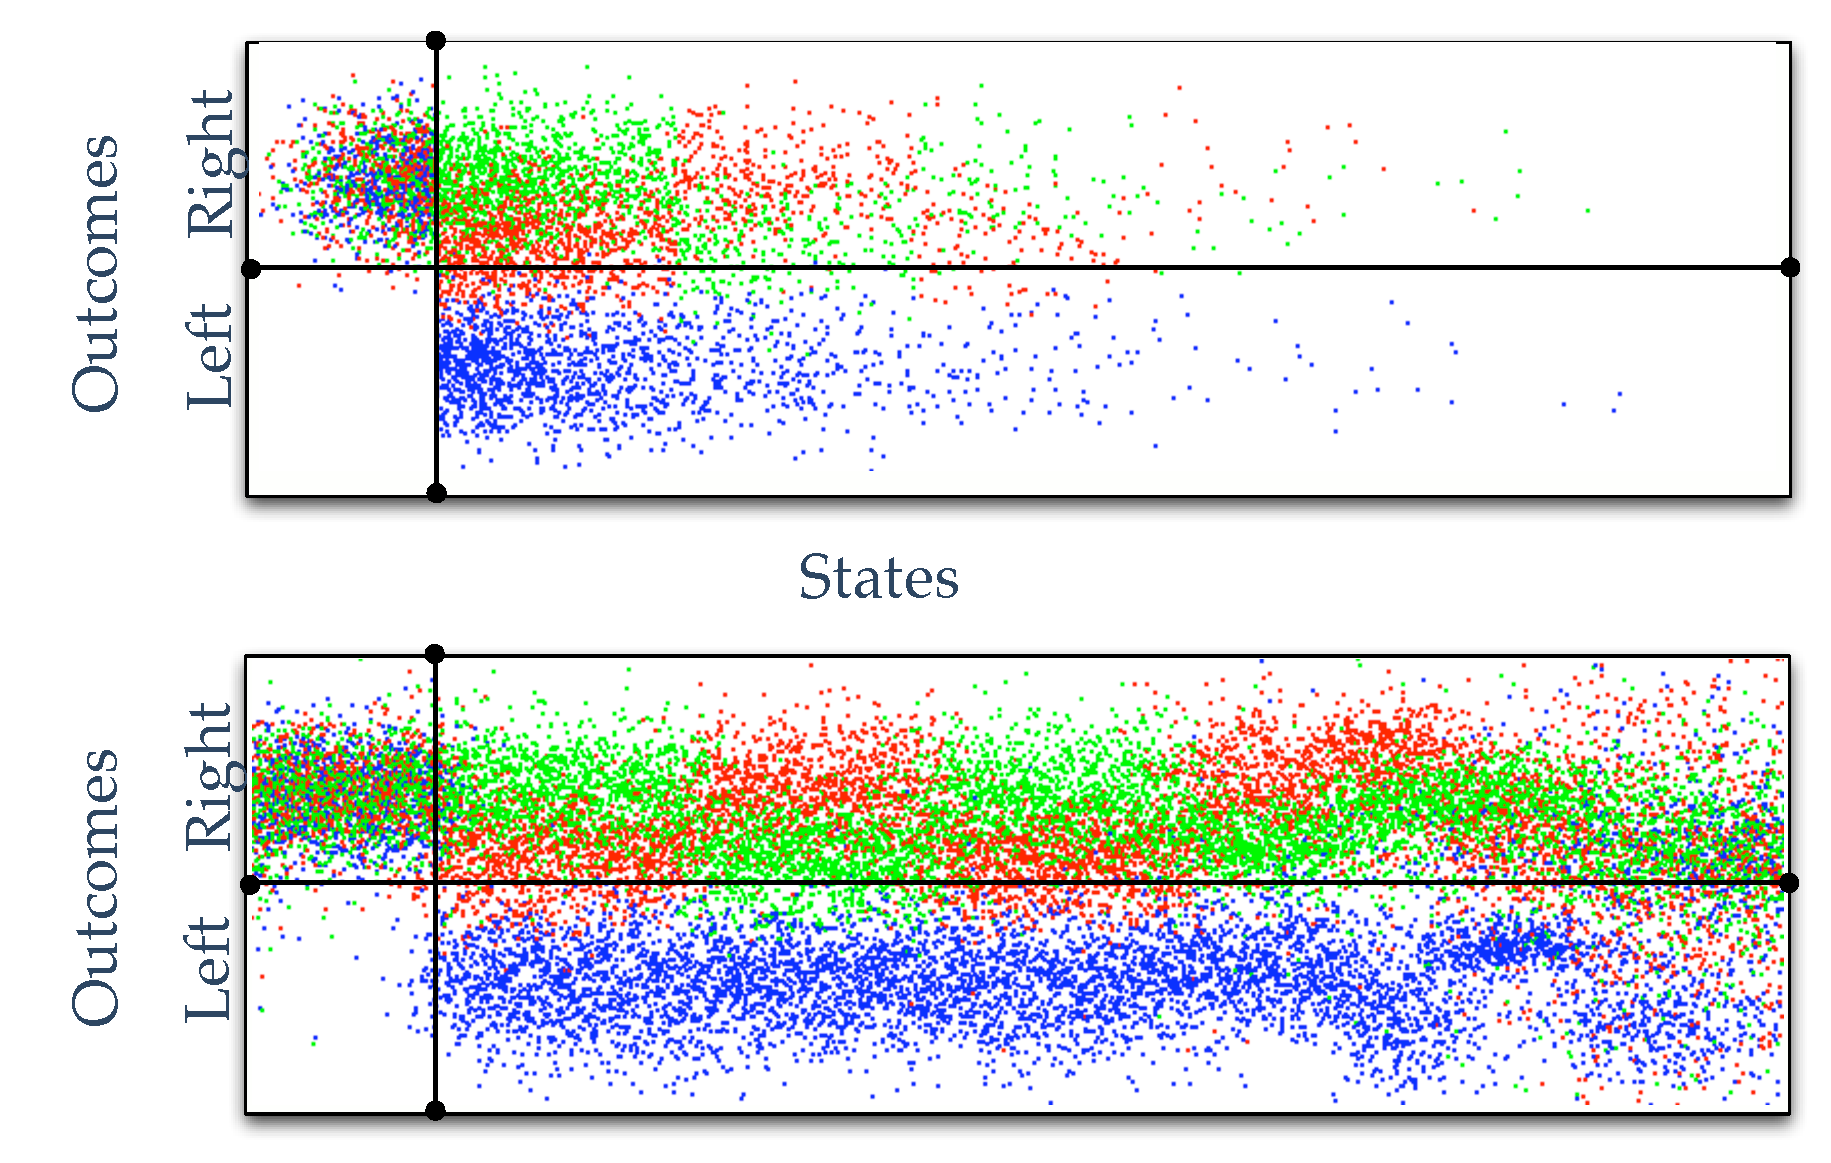
\includegraphics[width=0.9\linewidth]{figures/riverswim.pdf}
\caption{\env{Riverswim} is a simple environment where a fish tries to make its way up the river, and can take one of three actions: red, green, or blue. In these figures, the horizontal axis represents a state in the environment: further to the right means further up the river. The vertical axis represents a possible outcome: further up means that an action took the fish futher up the river, with a point on the origin meaning that the fish did not move. Each dot represents an action taken, with its horizontal position being where the fish was, and the vertical position being how far it moved. The top figure is experience in the actual environment; every dot represents an action that the agent took, and feedback it got from the environment. The bottom figure is experience sampled from the \prior{ROAR} posterior. As a human, one can see that it matches very closely the dynamics from the original environment, especially where there are more samples. Where there are fewer samples, to the right, \env{ROAR} has less to go on and its estimates are less accurate. However, because each sample is conditioned on previous samples, there are still visible clusters to the right. \env{ROAR} is making these up, and although they may be inaccurate, they are self-consistent and can be used to speculate about unexplored parts of the statespace without simply indicating that they are all drawn identically from the prior.}
\label{sec:models:riverswim}
\end{center}
\end{figure}


\section{Sample complexity}
\label{sec:models:complex}


Since a common subgoal for a reinforcement-learning agent is to learn a model, it is useful to quantify the sample complexity of a model in the first place. It is certainly true that there are some combinations of model priors and ``true'' models\footnote{That is, models from which the observations are sampled.} that do not allow learning of the model without an unreasonably large number of samples.

\begin{example}

Consider the coin flipping experiment in Section~\ref{sec:intro:coin-flipping}. Using a variable $x$ instead of the concrete likelihood $\frac{9990}{10000}$, we get the model
\begin{eqnarray}
\label{sec:models:eqn:coinbag}
\phi &=& \left\{\begin{array}{lll}
0.5 & \mbox{w.p.} & x,\\
1 & \mbox{w.p.} & 1-x,
\end{array}\right.\\
\rho &\sim&\phi,\\
H &\sim& \mbox{Binomial}(\rho, n).
\end{eqnarray}

For any given probability in Equation~\ref{intro:eqn:coinbag}, there is a number of heads-in-a-row, without any tails, that is required before the posterior indicates that the coin is more likely biased than not. The threshold will occur when $P(\rho=1|H=n,n)=P(\rho=0.5|H=n,n)$. If we substitute $x$ for $\frac{9990}{10000}$ in Equation~\ref{intro:eqn:coinbag}, this threshold gives us the relation
\begin{eqnarray}
x &=& \frac{1}{2^n+1}.
\end{eqnarray}
Given this relation, we can say something the sample complexity of a biased coin is with this prior.


With the coin flipping example, we give only two possibilities in the prior: double-headed or unbiased. These two coins are not $\epsilon$-close to each other, for any reasonable $\epsilon$, since the likelihood of \emph{heads} for the double-headed coin is $0.5$ away from that of the unbiased coin, and the same distance for tails. If the posterior has a probability of at least $\delta$ of sampling an unbiased coin after $B$ flips, the double-headed coin has a sample complexity greater than $B$, with respect to the prior in Equation~\ref{sec:models:eqn:coinbag}.

Choosing $\epsilon<0.5$, so that an unbiased coin is not considered an $\epsilon$-approximation of a double-headed coin, there is a relation between the number of samples $B$, the prior likelihood $x$, and the probability of failure $\delta$. We need to find $B$ such that the posterior likelihood for the double-headed coin is at least $1-\delta$. That is,
\begin{eqnarray}
\frac
 {P(\rho=1|H=B,n=B)}
 {P(\rho=\frac{1}{2}|H=B,n=B)}
&\geq&
\frac
 {1-\delta}
 {\delta},\\
 %
\frac
 {{B \choose B}1^B0^0 (1-x)} 
 {{B \choose B}{\frac{1}{2}}^B{\frac{1}{2}}^0 x}
&\geq&
\frac
 {1-\delta}
 {\delta},\\
 %
\frac
 {(1-x)} 
 {{\frac{1}{2^B}} x}
&\geq&
\frac
 {1-\delta}
 {\delta},\\
 %
 2^B(1-x)\delta 
 &\geq&
 (1-\delta)x,\\
 %
 2^B 
 &\geq&
\frac
 {(1-\delta)x}
 {(1-x)\delta},\\
%
B &\geq& \log_2\left(\frac
 {(1-\delta)x}
 {(1-x)\delta}
 \right).
\end{eqnarray}

Then, if we set $x=0.999$ and $\delta=0.001$, we find that $B\geq20$ is sufficient.


\end{example}

The rest of this section will attempt to formalize the concept of sample complexity for Bayesian machine learning.

\subsection{Sample complexity of the model for a stochastic function}

Given
\begin{itemize}
\item a set $X$,
\item a set $Y$,
\item a similarity metric $\sigma:X\times X\rightarrow[0,1]$,
\item any base value $x_0\in X$,
\item any vector of example values $\bar x \in X^n$ such that $\sum_{i=1}^n \sigma(x_0, \bar x_i) \geq B$,
\item a set of models $P$ with $\eta_0 \in P$,
\item a stochastic function $f_{\eta_0}:X\rightarrow\Pi(Y)$,
\item and some prior distribution $\phi \in \Pi(P)$ over models,
\end{itemize}
we say that a specific model $\eta_0 \in P$ has a sample complexity of $B$ with $\phi$ if the process
\begin{eqnarray}
\bar y_i &\sim& f_{\eta_0}(\bar x_i),\\
\tilde\eta &\sim& \phi|(\bar x, \bar y),
\end{eqnarray}
results in the condition
\begin{eqnarray}
\forall_{y\in Y}|f_{\tilde\eta}(y|x_0)-f_{\eta_0}(y|x_0)| &\leq& \epsilon
\end{eqnarray}
holding with probability at least $1-\delta$.

Note that this must hold true for any $\bar x$, and that this $\bar x$ is chosen before-hand.

This guarantee can easily be adapted for a discrete set $X$ whose members cannot be generalized. In this case, the similarity metric $\sigma$ is the Kronecker delta, where the result is $1$ if the two values are identical, and $0$ otherwise. With this metric, there must be at least $B$ examples of $x_0$ in the set of example values. 


To map this setting to the coin-flip example above, consider the set $X$ to be the set of all coins, double-headed or not. Then, we need examples of flips from the coins in that set such that the coins are sufficiently similar to the one we're thinking about, $x_0$. In this case, we only care about coins that are exactly the coin we're trying to estimate, so we need $B$ examples of that coin. The set $Y$ will be the set $\{\mbox{heads},\mbox{tails}\}$, and $\eta_0$ is a model indicating that coin $x_0$ is double-headed. As a result, flipping the double-headed coin, or calling $f_{\eta_0}(x_0)$, should result in heads each time.

Intuitively, if a model has a sample complextiy of $B$, then we only need $B$ evidence (according to the similarity metric $\sigma$) at a given point to have a posterior sample be $\epsilon$-accurate at that point with probability $1-\delta$.

In Chapter~\ref{sec:boss}, I will show that this sample complexity guarantee is a sufficient condition for the posterior accuracy conditions in the analysis of a model-based Bayesian reinforcement-learning algorithm. In the later sections of this chapter, I will describe how to fit different types of MDPs, and their priors, to this guarantee.

\subsection{Sample complexity of the transition function for a discrete-state, discrete-action MDP}

An MDP $m_0$ can be considered the model for a stochastic function. The transition function $T_{m_0}:S \times A \rightarrow S$ is a function using the MDP components as its model. Specifically, $T_{m_0}(s,a)$ is a multinomial distribution parameterized by an unknown $\theta_0^{s,a}$ vector, which has a prior distribution $\phi$. The goal is to then evaluate the sample complexity of a particular vector $\theta_0^{s,a}$ is, with samples from the stochastic function $T_{m_0}(s,a) = \mbox{Mult}(\theta_0^{s,a})$.

Given
\begin{itemize}
\item $X$ is the set of all state-action pairs $S\times A$,
\item $Y$ is the set of states $S$,
\item $x_0$ is some state-action pair $(s_0, a_0)$,
\item $\bar x$ is any vector of state-action pairs that contains at least $B$ instances of $(s_0,a_0)$,
\item $P$ is the set of all possible multinomials for each of the state-action pairs in the MDP,
\item and $f_{\eta_0}$ is $T_{m_0}$, or the transition function of the true MDP $m_0$,
\end{itemize}
when the process
\begin{eqnarray}
s'_i &\sim& \mbox{Mult}(\theta_0^{s_i a_i}),\\
\tilde \theta_{s,a} &\sim& \phi|(s_1,a_1,s'_1),(s_2,a_2,s'_2),...,(s_n,a_n,s'_n),
\end{eqnarray}


results in a posterior sample satisfying
\begin{eqnarray}
\forall_{s'\in S} |\tilde\theta_{s_0 a_0}(s') - \theta^0_{s_0 a_0}(s')| & \leq & \epsilon,
\end{eqnarray}
with probability at least $1-\delta$, we can say that the MDP $m_0$'s transition function has a sample complexity of $B$.

\subsubsection{Sample complexity of an MDP using the Flat Dirichlet Multinomial}

The \prior{Flat Dirichlet Multinomial} prior, or \prior{FDM}, described in Chapter~\ref{sec:models}, is one of the simplest priors for a discrete-state, discrete-action MDP. With the \prior{FDM} prior, the transition function for each state is treated as an independent problem where the parameter $\theta_0$ is learned from a set of samples from $\mbox{Mult}(\theta_0)$, and $\theta \sim \mbox{Dir}(\alpha)$.

We can then simplify the analysis of a model with the \prior{FDM} prior's sample complexity to that of the sample complexity of some random simplex $\theta_0$ with a Dirichlet prior.

\begin{example}

Let $\alpha=(1, 1)$ and $\theta_0=(\frac 1 2, \frac 1 2)$. This problem is the same as the sample complexity of an unbiased coin with a uniform prior over its bias (that is, an unbiased coin is just as likely as a double-headed coin, which is just as likely as a coin that lands heads $2/3$ of the time, etc.).

We can resolve the question of the sample complexity for this prior by answering the question of how many times we need to flip this biased coin such that our posterior samples are accurate.

Let $\epsilon = 0.1$ and $\delta = 0.1$. Then, for the unbiased coin to have a sample complexity of $B$, we need to choose a $B$ that is high enough so that $90\%$ of the time when we perform the experiment of flipping the coin $B$ times and sampling from the posterior, we get a coin with a heads likelihood in $[0.4,0.6]$ and a tails likelihood in $[0.4,0.6]$.

Since the Multinomial distribution with two outcomes is the Binomial distribution, and the Dirichlet distribution on the two-dimensional simplex is the Beta distribution, we can use those distributions in our analysis. That is, given the process
\begin{eqnarray}
H &\sim& \mbox{Bin}(\rho=0.5, B),\\
\tilde \rho &\sim& \mbox{Dir}(\alpha=(H+1, \beta=B-H+1)),\\
\end{eqnarray}
choose a value $B$ such that
\begin{eqnarray}
P(0.4\leq \tilde \rho\leq 0.6)&\geq& 1-\delta,\\
%
\begin{array}{ll}
&\sum_{H=0}^B \mbox{Bin}(H|\rho=0.5,n=B)\\
\cdot &\int_{\tilde \rho=0.4}^{0.6} \mbox{Beta}(\rho|\alpha=H+1,\beta=B-H+1),
\end{array}
&\geq& 1-\delta\\
%
\label{sec:guarantees:fdm-likelihood}
\sum_{H=0}^B {B \choose H} \frac 1 {2^B}
\left[
 \begin{array}{l}
  I_{\min({1,{\frac 1 2 + \epsilon}})}(H+1,B-H+1)\\
  -I_{\max({0,{\frac 1 2 - \epsilon}})}(H+1,B-H+1)
 \end{array}
\right]&\geq& 1-\delta,
\end{eqnarray}
where $I_p(\alpha,\beta)$ is the regularized incomplete gamma function, and $\int_0^p\mbox{Beta}(p|\alpha,\beta) dp = I_p(\alpha,\beta)$.

The smallest $B$ that satisfies Equation~\ref{sec:guarantees:fdm-likelihood} can be found numerically, and happens to be $21$. As a result, the unbiased coin has a sample complexity of $B=20$ with the $\mbox{Beta}(1,1)$ prior, for $\epsilon=0.1$ and $\delta=0.1$.

\end{example}

In general, for any hyperparameter $\alpha$, set of states $S$, and true model $\theta_0$,, we can relate $B$, $\epsilon$ and $\delta$ with the following equation:
\begin{eqnarray}
\sum_{\bar {s'}:||\bar {s'}||_1 = B} \limits
 \mbox{Mult}(\bar {s'}|\theta_0,B)
 \int_{\theta:||\theta-\theta_0||_1 \leq \epsilon}\limits
  \mbox{Dir}(\theta|\alpha+\bar{s'})
  d\theta
&\geq& 1-\delta.
\end{eqnarray}
Although the analysis is difficult, numerical techniques can be used to find the smallest value $B$ for a given $\epsilon$ and $\delta$.

\subsection{Sample complexity of the prior}

So far, this chapter has discussed the sample complexity of a particular ``true'' model for a given prior.

That is, if we start with $\epsilon$, $\delta$, $\phi$, and $\eta_0$, we can imagine a function $B(\eta_0,\phi,\epsilon,\delta)$ that tells us how many samples are required to learn that model, given our accuracy constraints, desired likelihood of success, and prior distribution.

It also makes sense to talk about the expected sample complexity, given a prior. The sample complexity of a prior is
\begin{eqnarray}
L(\phi,\epsilon,\delta)
&=&
\int_{\eta_0} \phi(\eta_0) B(\eta_0,\phi,\epsilon,\delta) d\eta_0.
\end{eqnarray}

In other words, the sample complexity of a prior is the expected sample complexity of a model sampled from that prior.

Although the sample complexity is difficult to express exactly, it is related to the probability of success. If, with $\bar x:\sum_i \sigma(x_0,{\bar x}_i)\geq B$,
\begin{eqnarray}
\label{sec:guarantees:prior-learnability}
\int_{\eta_0}\limits
 \phi(\eta_0) \left[
 \int_{\bar y} \limits
  f_{\eta_0}(\bar y|\bar x) \left[
  \int_{\tilde\eta}\limits
   \phi(\tilde\eta|(\bar x, \bar y))
   \mathbb{1}(||\tilde\eta-\eta_0||\leq\epsilon)
  \ d\tilde\eta \right]
 \ d\bar y \right]
\ d\eta_0
&\geq&
1-\delta.
\end{eqnarray}
In english, first we pick a ``true'' model $\eta_0$ according to the prior $\phi$. Then, we make some observations $\hat y$ from the world created by $\eta_0$. Once we have the ``true'' model and the observations, we see how many models are $\epsilon$-close to the ``true'' model, weighted according to their posterior likelihoods.


\begin{example}

\label{sec:guarantees:beta-bin}

We can find the sample complexity of the Beta-Binomial model,
\begin{eqnarray}
\label{sec:guarantees:eqn:beta-bin-beta}
\rho &\sim& \dBeta(\alpha,\beta),\\
\label{sec:guarantees:eqn:beta-bin-bin}
H &\sim& \dBin(\rho_0, B).
\end{eqnarray}

The Beta-Binomial prior's $\rho$ parameter has a sample complexity of $B$ if
\begin{eqnarray}
\begin{array}{l}
\int_{\rho_0} \dBeta(\rho_0|\alpha,\beta)
 \sum_{H=0}^B \dBin(H|\rho_0,B)\\
 \cdot
  \int_{\tilde\rho=\rho_0-\epsilon}^{\rho_0+\epsilon} \dBeta(\tilde\rho|\alpha+H,\beta+B-H)
   d\tilde\rho \
  d\rho_0
  \end{array}
&\geq& 1-\delta,\\
%
\label{sec:guarantees:eqn:beta-binomial-learnable}
\begin{array}{l}
\int_{\rho_0} \dBeta(\rho_0|\alpha,\beta)
 \sum_{H=0}^B \dBin(H|\rho_0,B)\\
  \cdot \left[
   I_{\rho_0+\epsilon}(\alpha+H,\beta+B-H)
   -I_{\rho_0-\epsilon}(\alpha+H,\beta+B-H)
  \right]
  d\rho_0
\end{array}
&\geq& 1-\delta,
\end{eqnarray}
where $I_x(a,b)=I_{\max(0, \min(1, x))}(a,b)$ is the regularized incomplete gamma function.

For a given $\epsilon$, $\delta$, $\alpha$, and $\beta$, the smallest $B$ that satisfies Equation~\ref{sec:guarantees:eqn:beta-binomial-learnable} can be found numerically. Table~\ref{sec:guarantees:table:beta-bin} lists several example sample complexities for different values of $\epsilon$ and $\delta$, and different prior parameters.


\begin{table}
\caption{Sample complexity for the Beta-Binomial. Using the model from Section~\ref{sec:guarantees:beta-bin}, the posterior for the latent variable $\rho$ is $\epsilon$-accurate with probability at least $1-\delta$ if $B$ is above some threshold. This table gives examples of the relations between the model hyperparameters, $\epsilon$, $\delta$, and $B$. }
\label{sec:guarantees:table:beta-bin}
\center{\small
\begin{tabular}{rccl}
       $(\alpha,\beta)$ & $\delta$ & $\epsilon$ & lowest $B$ \\
$(1,1)$ &  $0.1$ & $0.1$ & 91 \\
$(50,50)$ &  $0.1$ & $0.1$ & 31\\
$(100,100)$ &  $0.1$ & $0.1$ & 0 \\
$(1,5)$ &  $0.1$ & $0.1$ & 61 \\
$(5,25)$ &  $0.1$ & $0.1$ & 43\\
$(10,50)$ &  $0.1$ & $0.1$ & 13
\end{tabular}
}\\
\end{table}

\end{example}


%
\ifperchapterbib%
For the convenience of the reader, a list of references is provided at the end of each chapter (where applicable).
\ifendbib%
A bibliography containing all cited references is included at the \hyperref[sec:bibliography]{end of the dissertation}.
\else\fi% end ifendbib
\cbend%
\else\fi% end ifperchapterbib